\chapter{Tests conducted}

\section{Indirect filling of on-board DRAM}

To check access of the host to the full 4GB on board DRAM Memory through a Memory Address Translator Block which Translates a read/write
request in form of two AXI slave register writes to an AXI Master request on the onboard AXI interconnect. It employs 3 registers to
accommodate address, data and type of request respectively. Figure~\ref{MAT flow} shows the flow for this indirect access to the on-board
DRAM through the Memory Address Translation block. More details have been provided in section~\ref{MAT block} regarding this block.

\begin{figure}[H]
\centering
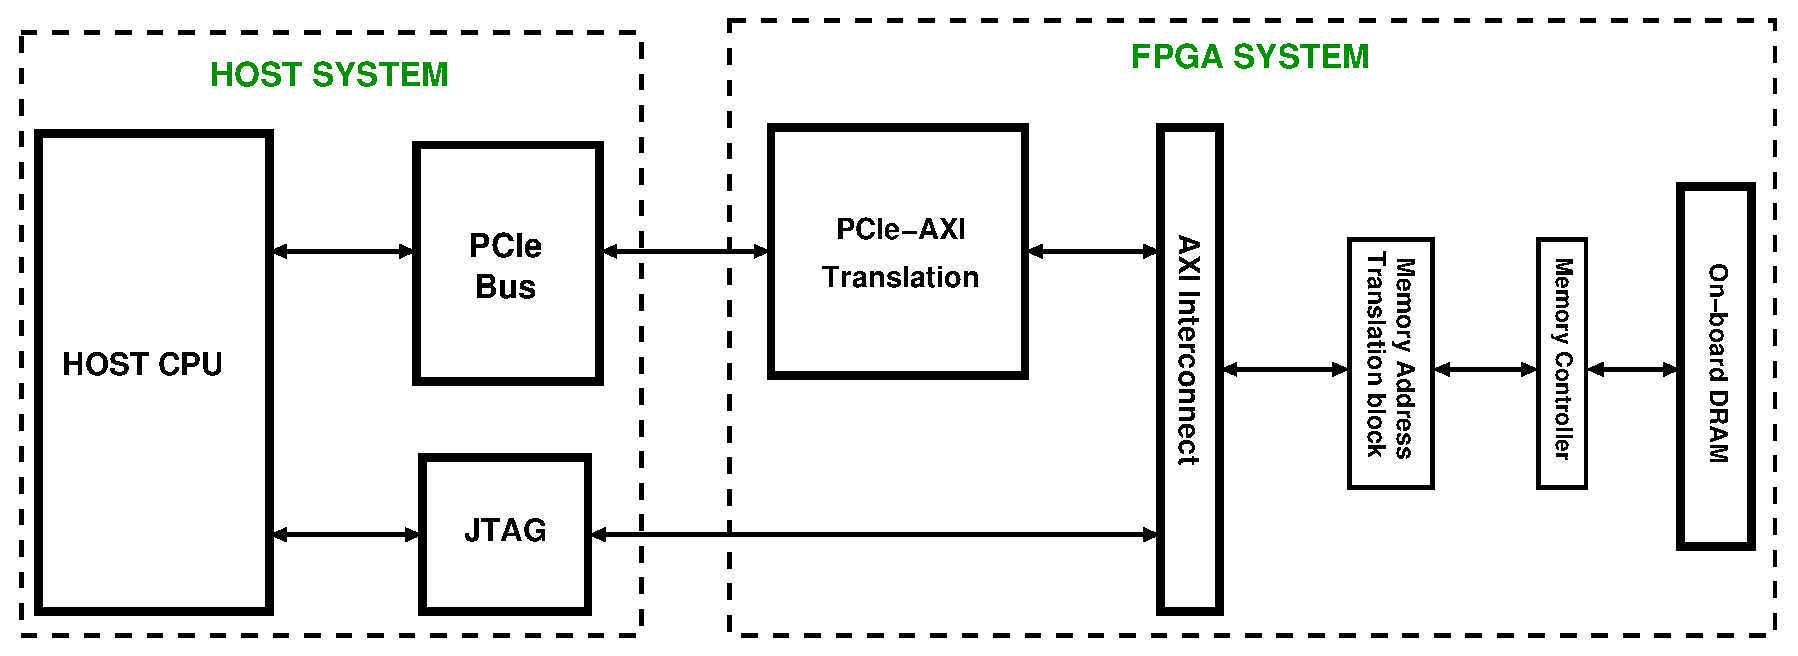
\includegraphics[width=\textwidth]{eps_pdf_sources/ajit_fpga/Tests_conducted/MAT}
\caption{Indirect memory channel from host to AJIT}
\label{MAT flow}
\end{figure}

\subsection{Results}

In order to write the whole 4GB memory through this block took around 45 minutes since in order to perform a single write to the on board
DRAM through this peripheral we need to perform 3 writes to this block including write address, write data and the type of request as write
into the AXI Slave registers of this block.

\section{March test on memory}

\subsection{What is March Test?}

A march test consists of a finite sequence of march elements. A march element is A finite sequence of Read and/or Write operations applied
to every cell in memory in either increasing address order (cell 0 to cell n-1) or decreasing address order (cell n-1 to cell 0). All
operations of a march element are done before proceeding to the next address. The march tests are a preferred method for RAM testing-Linear
complexity, regularity, and symmetry.

\subsection{Fault Models}
\begin{table}[H]
\begin{tabular}{c | m{0.7\textwidth}}
\hline
Fault Models & Description \\
\hline
Stuck-At Fault & The logic value of a line is always \textbf{0 or 1}\\
Transition Fault & A cell or a line that fails to undergo a $0 \rightarrow 1$ or a $1 \rightarrow 0$ transition \\
Coupling Fault & A write operation to one cell changes the content of a second cell other cells in the memory \\
NPS Fault & The content of a cell, or the ability to change its content, is influenced by the contents of some\\
Address Decodes Fault & With a certain address no cell will be accessed, a certain cell is never accessed, with a certain address multiple
cells are accessed simultaneously, and a certain cell can be accessed by multiple addresses
\end{tabular}
\caption{Fault Models}
\end{table}

\textit{NPS}: Neighbourhood Pattern Sensitive

\subsection{Our Implementation}
Here we perform the standard March test on the on board DRAM memory by accessing it from the host using the 6 PCIe BARS created as PCIe
resources on the /sys path of Linux. We implement the \textbf{March X} algorithm because it
is an $O(n)$ time algorithm and covers most of the basic faults.

\begin{algorithm}
\caption{March X algorithm}\label{March X}
\begin{algorithmic}[1]
\State Step 1: \textbf{write} 0 with up addressing order;
\State Step 2: \textbf{read} 0 and \textbf{write} 1 with up addressing order;
\State Step 3: \textbf{read} 1 and \textbf{write} 0 with down addressing order;
\State Step 4: \textbf{read} 0 with down addressing order;
\end{algorithmic}
\end{algorithm}

\subsection{Faults covered}
The above algorithm covers Address Decoder Faults, Stuck at Faults, Transition Faults and some coupling faults.

\subsection{Timing Results}

The below table consists of the time taken by the host to conduct the March test on each bar of the on-board memory.

\begin{table}[H]
\centering
\begin{tabular}{c | c}
\hline
BAR ID & Time Taken(in sec) \\
\hline
BAR0 & 59.658342534 \\
BAR1 & 59.640203597 \\
BAR2 & 59.607970220 \\
BAR3 & 59.611384216 \\
BAR4 & 59.690874289 \\
BAR5 & 59.722889924
\end{tabular}
\caption{Timing Results}
\end{table}
